% PROCESS-BASED & DATA-DRIVEN
As elsewhere, in hydrology one distinguishes between physical process-based and purely data-driven modeling approaches \cite{Physics:Singh2002,Physics:Todini2007,Physics:Todini2011}.
Even if a model is primarily based on physical principles, the parameters and predictions have to be respectively calibrated and corrected in conjunction with experimental data.
This is the goal of this chapter.
% INITITAL SITUATION
The physics-oriented hydrological model under consideration predicts the outflow from an urban drainage basin in a precipitation event.
Dynamical simulations of the runoff are based on a series of rainfall measurements.
Some further model inputs are unknown and shall be calibrated with time series data of the outflow.
Bounds of these unknowns are established and their prior distributions are prescribed.
If the model could be run for arbitrarily chosen values of the inputs, the uncertain parameters could be identified with the methods previously discussed in this thesis.
However, this is not the case, because the model is not available to us in an executable form.
\par % BLACK-BOX SCENARIO
We only have the results of a limited number of simulator runs that were performed for certain rainfall data and uniformly varying values of the unknown parameters.
In this situation we have to construct an operational emulator first.
The originally performed model runs are fed into a metamodeling procedure for that purpose.
After a surrogate model is obtained, one can use it in order to ``interpolate'' between the design points in continuous fashion.
This way the simulator output can be at least computed approximately for arbitrary values of the unknowns.
Subsequently Bayesian inference proceeds as usual.
\par % MODEL AND DATA
We start with a brief description of the urban drainage model and the measurement data.
More details can be taken from the fourth chapter of \cite{Hydro:Machac2015:PhD}.
% STORM WATER MANAGEMENT MODEL
The storm water management model (SWMM) is a dynamic rainfall-runoff simulation program for urban areas \cite{Hydro:SWMM2015}.
It can be used to predict the runoff from a catchment area during and shortly after a rainfall event.
% ADLISWIL CATCHMENT
A model of the drainage basin of Adliswil, a municipality in the canton of Z\"{u}rich in the northeast of Switzerland, was created with the SWMM.
In \cref{fig:Hydro:OSM:Adliswil} a map is provided that shows the surrounding area of the size \(\unit[5]{km} \times \unit[3]{km}\).
The SWMM implementation models about \(\unit[160]{ha}\) of this area, i.e.\ approximately ten percent.
Roughly speaking, this SWMM implementation uses one hundred sub-catchments that are linked through five hundred channels.
% FIGURE: ADLISWIL MUNICIPALITY
\begin{figure}[htbp]
  \centering
  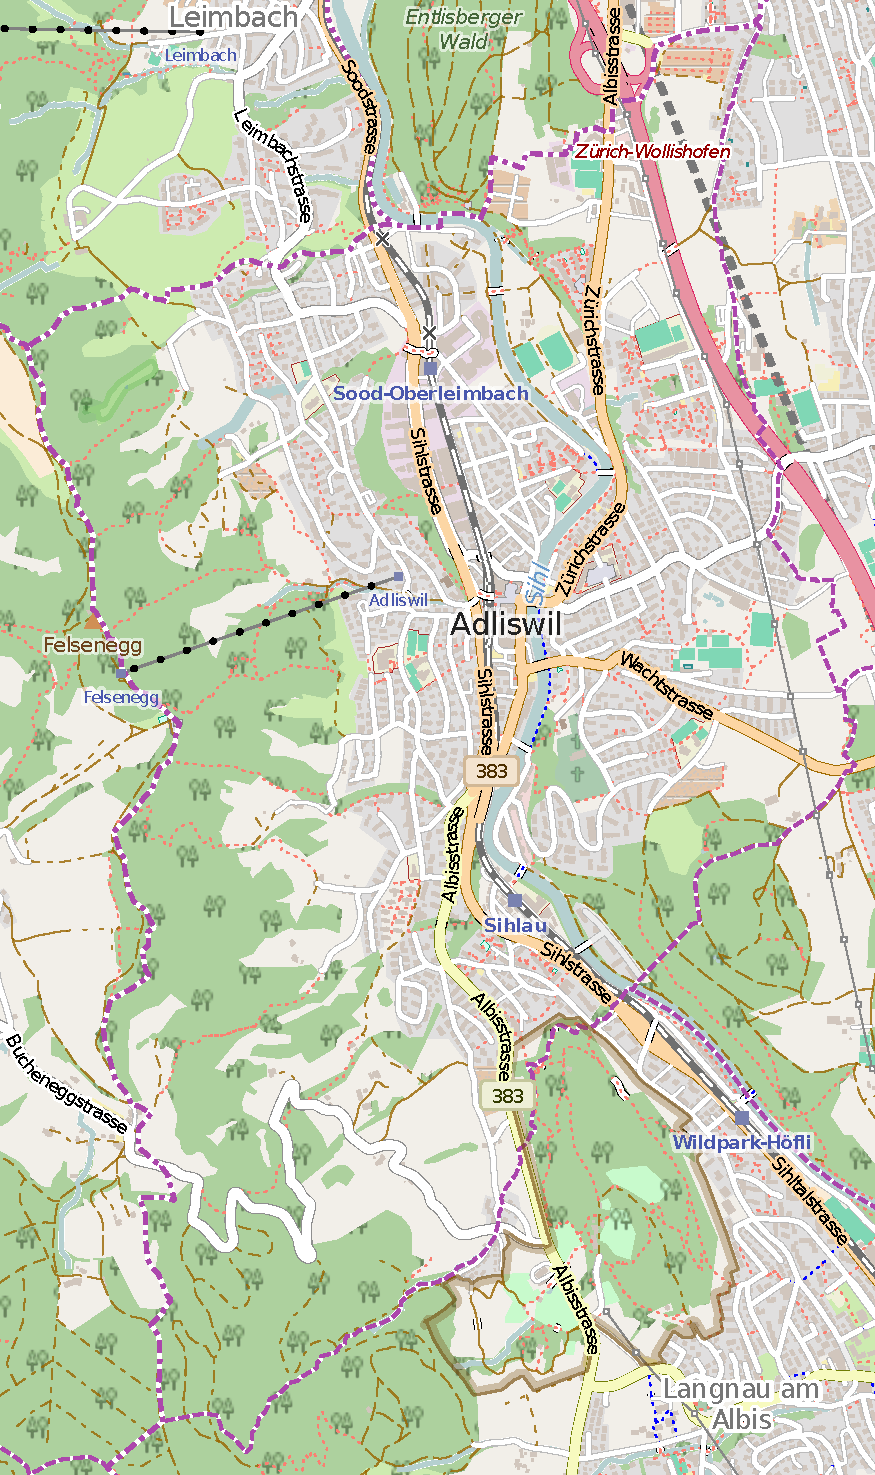
\includegraphics[height=\HYDROmapHeight]{fig_Hydro_OSM_Adliswil}
  \caption[Adliswil, Switzerland (1:50000)]{Adliswil, Switzerland (1:50000).
           From \href{https://www.openstreetmap.org}{OpenStreetMap} under \href{https://creativecommons.org/licenses/by-sa/2.0/}{CC BY-SA 2.0}.
           \textcopyright{} \href{https://www.openstreetmap.org/copyright}{OpenStreetMap contributors}.}
  \label{fig:Hydro:OSM:Adliswil}
\end{figure}
\par % AVERAGE PARAMETERS
All sub-catchments and interconnections have their own unknown parameters.
This amounts to a fairly large number of unknowns that is reduced by considering spatial averages only,
i.e.\ physical quantities of the same type are averaged over the sub-catchments or channels.
Moreover, the parameter classes are normalized so as to be dimensionless and to lie in between reasonable bounds.
A compilation of the obtained scaled parameters \(x_i \in \mathcal{D}_{x_i}\) for \(i=1,\ldots,8\)
and their bounded domains \(\mathcal{D}_{x_i} = [\underline{x}_i,\overline{x}_i]\) is presented in \cref{tab:Hydro:Parameters} below.
The physical quantities described and their unscaled spatial averages are also provided.
While the first seven parameters relate to the sub-catchments, only the last one characterizes the pipes.
% TABLE: MODEL PARAMETERS
\begin{table}[htbp]
  \caption[Hydrological model parameters]{Hydrological model parameters.}
  \label{tab:Hydro:Parameters}
  \centering
  \begin{tabular}{llll}
    \toprule
    \(x_i\) & \(\mathcal{D}_{x_i}\) & Physical parameter & Spatial average \\
    \midrule
    \(x_1\) & \([0.5,1.1]\) & Percentage of the impervious area                            & \(\unit[36]{\%}\) \\
    \(x_2\) & \([0.5,1.5]\) & Characteristic width of the overland flow path               & \(\unit[35.7]{m}\) \\
    \(x_3\) & \([0.5,1.5]\) & Slope of the sub-catchments                                  & \(\unit[11.4]{\%}\) \\
    \(x_4\) & \([0.5,1.5]\) & Depression storage height of the impervious area             & \(\unit[2]{mm}\) \\
    \(x_5\) & \([0.5,1.5]\) & Manning roughness coefficient of the impervious area         & \(\unit[0.12]{s \cdot m^{-1/3}}\) \\
    \(x_6\) & \([0.5,1.5]\) & Depression storage height of the pervious area               & \(\unit[2]{mm}\) \\
    \(x_7\) & \([0.5,1.5]\) & Percentage of the impervious area without depression storage & \(\unit[19.04]{\%}\) \\
    \(x_8\) & \([1.0,1.5]\) & Manning roughness coefficient of the channels                & \(\unit[0.012]{s \cdot m^{-1/3}}\) \\
    \bottomrule
  \end{tabular}
\end{table}
\par % OBSERVATIONAL DATA
A single \(15\)-hour rainfall event is considered that had occurred on May 28, 2013.
Time is denoted as \(t\) in the following.
The experiment extends over a period with \(t / \unit[120]{s} \in [0,600]\).
Measurements of the varying rainfall intensity \(I\) and the catchment outflow \(Q\) are taken in regular intervals of two minutes over the full duration.
For \(i=0,\ldots,600\) the time instances of the observations are denoted as \(t_i\).
Both rainfall and outflow measurements were made at single locations within the drainage basin, e.g.\ the outflow was measured at the wastewater treatment plant.
In \cref{fig:Hydro:Data} the available data are summarized.
The observations of the rainfall intensity \(I(t_i)\) are indicated by the black dots in \cref{fig:Hydro:Data:Rainfall}.
Similarly, the recorded outflows \(Q(t_i)\) at the sewage treatment plant are shown in \cref{fig:Hydro:Data:Outflow}.
\par % EXPERIMENTAL DESIGN
Beyond the observational data just described, the results of approximately two thousand runs of the SWMM simulator are available.
These will constitute the training runs for the computation of the surrogate model in the next section.
They were conducted for the given rainfall data shown in \cref{fig:Hydro:Data:Rainfall} and uniformly distributed values of the uncertain hydrological parameters.
A hundred trajectories from these computer simulations are depicted in \cref{fig:Hydro:Data:Outflow}.
They can be compared to the actually measured runoffs in the same plot.
\par % DISCUSSION
The model manages to capture the main trends and characteristics of the data.
In the time interval \(t / \unit[120]{s} \in [150,200]\) it seems to slightly underpredict the outflow, though.
An even stronger systematic discrepancy is detected for the time span \(t / \unit[120]{s} \in [250,500]\) during which the outflow is overpredicted.
It is also noticed that the model predictions for different values of the uncertain inputs do not differ significantly,
i.e.\ they cannot be discriminated very well by their ability to trace the data.
This is especially obvious in the second half of the experiment with \(t / \unit[120]{s} \in [300,600]\).
Here, the mismatch between the data and the model predictions is apparently dominated by systematic errors and random noise, rather than by variations of the model inputs.
% FIGURES: EXPERIMENTAL DATA/DESIGN
\begin{figure}[htbp]
  \centering
  \begin{subfigure}[b]{\HYDROsubWidth}
    \centering
    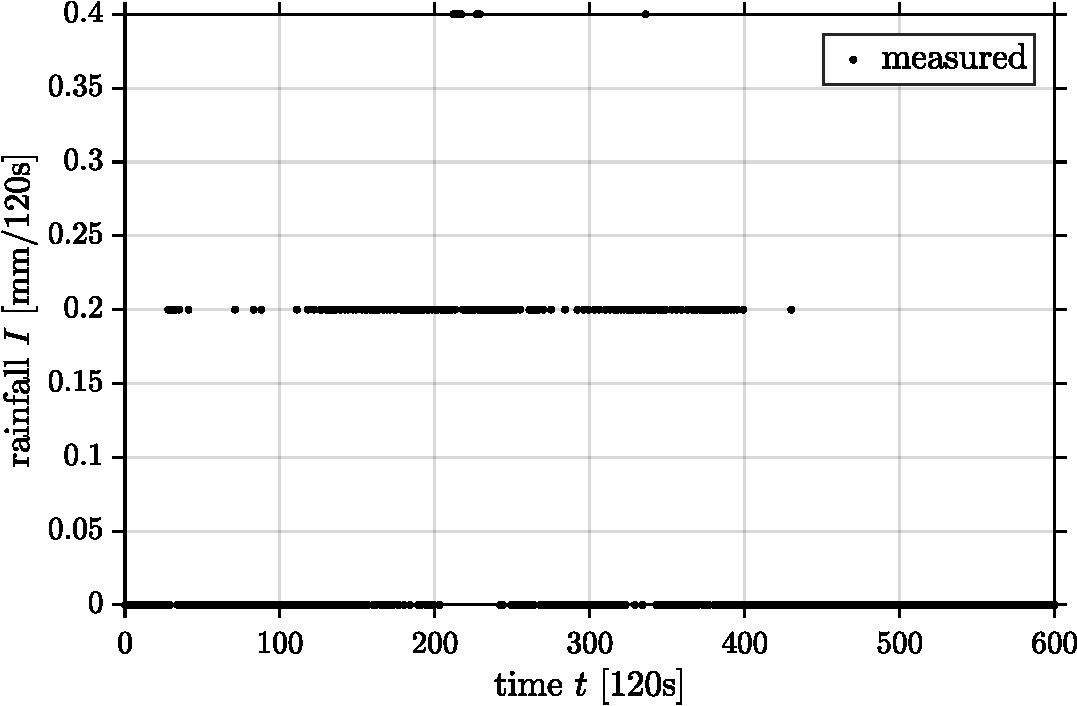
\includegraphics[height=\HYDROfigHeight]{fig_Hydro_Data_Rainfall}
    \caption{Rainfall intensity data.}
    \label{fig:Hydro:Data:Rainfall}
  \end{subfigure}\hfill%
  \begin{subfigure}[b]{\HYDROsubWidth}
    \centering
    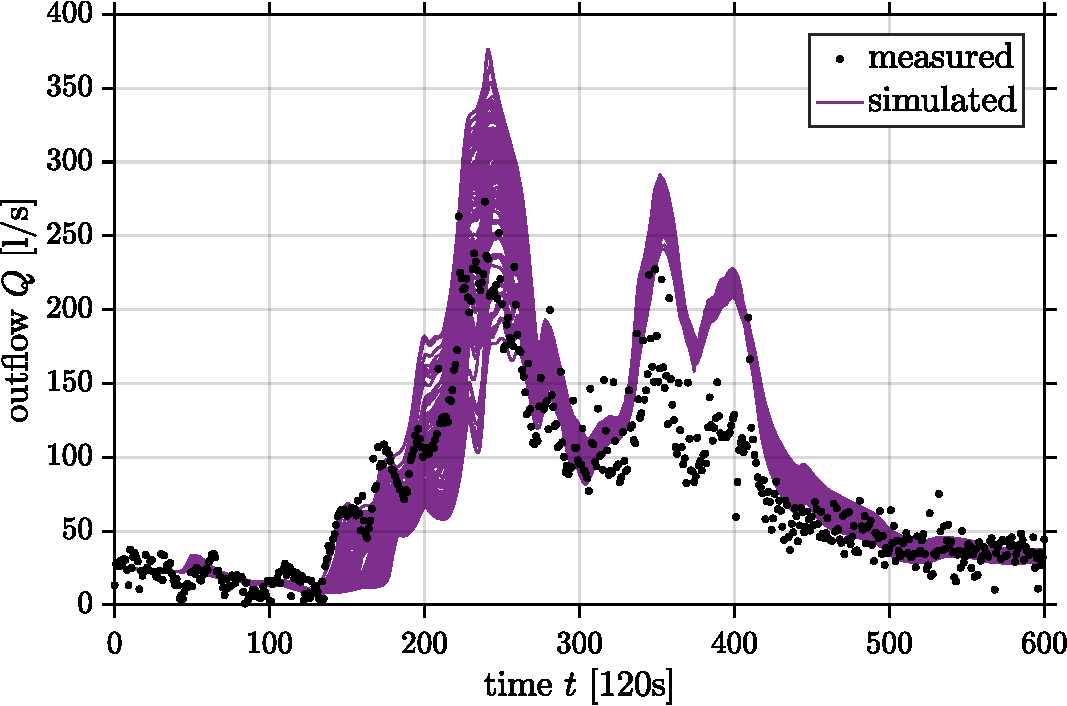
\includegraphics[height=\HYDROfigHeight]{fig_Hydro_Data_Outflow}
    \caption{Observed and simulated outflow.}
    \label{fig:Hydro:Data:Outflow}
  \end{subfigure}%
  \caption[Experimental data]{Experimental data.}
  \label{fig:Hydro:Data}
\end{figure}